\newpage
\section{Data Preprocessing}


%1. 。。。。。。数据全部缺失，不予考虑。
%2. 对数据测试的特点，如周期等进行分析。
%3. 。。。。。。数据残缺，根据数据挖掘等理论根据。。。。。变化趋势进行补充。
%4. 对数据特点（后面将会用到的特征）进行提取.
%用。。。。。。。软件聚类分析和各个不同问题的需要，采得。。。组采样，每组5-8个采样值。将采样所对应的特征值进行列表或图示。
%根据数据特点，对总体和个体的特点进行比较，以表格或图示方式显示。

本研究仅使用题目给定的DWTS官方赛季周度数据表。为确保后续推断（Q1）与机制对比/仿真（Q2--Q4）在同一数据口径下进行，我们首先将原始宽表转换为“周度面板（weekly panel）+ 赛季层特征（season features）”两张规范化数据集，并进行一致的缺失与异常处理。

\subsection{Data sources and canonicalization}
\begin{enumerate}[
    label = (\arabic*),
    itemindent = 0pt,
    labelindent = \parindent,
    labelwidth = 2em,
    labelsep = 5pt,
    leftmargin = 4.5em
    ]
    \item \textbf{字段解析与类型规范化：}将赛季$\times$周$\times$选手作为唯一键，统一数值字段（评委分、周平均分等）的类型；对字符串字段（选手名、机制名等）去除多余空格并标准化。
    \item \textbf{缺失与退出处理：}对明确“退出/退赛/淘汰”的记录在周度面板中标注退出周；对后续周的缺失分数不做插补（避免引入未来信息），仅用于“在场/不在场”状态更新。
    \item \textbf{一致性检查：}对每周在场人数、淘汰人数、分数范围进行基础审计，保证不存在明显的逻辑冲突（例如同一周多次淘汰、在场选手分数缺失占比异常等）。
\end{enumerate}

\subsection{Feature construction for downstream tasks}
在周度面板中，我们构造了以下关键特征（在Q1--Q4反复使用）：
\begin{enumerate}[
    label = (\arabic*),
    itemindent = 0pt,
    labelindent = \parindent,
    labelwidth = 2em,
    labelsep = 5pt,
    leftmargin = 4.5em
    ]
    \item \textbf{评委维度：}当周评委总分与其在当周的百分位/名次（用于“评委信号”）。
    \item \textbf{观众维度（可观测代理）：}由当周淘汰结果与评委信号共同约束，形成观众偏好强度的可推断结构（用于Q1的后验推断与不确定性量化）。
    \item \textbf{机制相关指标：}针对Percent与Rank两种投票合成方式，构造每周的机制得分、相对差异、以及跨周可比较的度量。
\end{enumerate}

为直观展示数据结构与“评委信号---观众结果”之间的关系，我们给出评委分与观众偏好推断信号的散点示意（图\ref{fig:q1_judge_vs_fan_scatter}）。该图既是数据探索的入口，也用于验证后续模型的方向性是否符合常识（例如评委分高但仍被淘汰的周，往往对应更强的观众偏好差异）。

\begin{figure}[H]
    \centering
    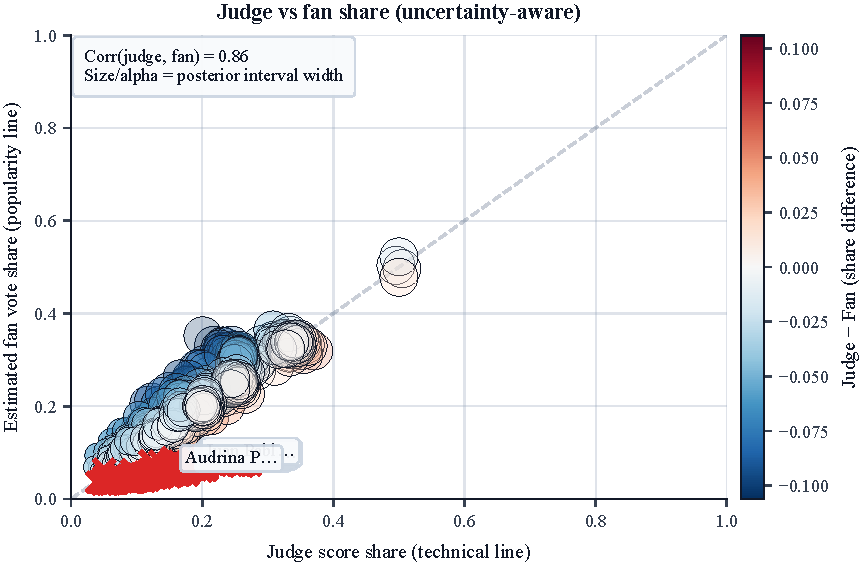
\includegraphics[width=0.92\linewidth]{../outputs/figures/q1/pdf/q1_judge_vs_fan_scatter.pdf}
    \caption{数据结构示意：评委分与观众偏好信号的关系（用于后续Q1推断与诊断）。}
    \label{fig:q1_judge_vs_fan_scatter}
\end{figure}
